\chapter{Experimental Design}

Lorem ipsum dolor sit amet, consectetur adipiscing elit, sed do eiusmod tempor incididunt ut labore et dolore magna aliqua. Ut enim ad minim veniam, quis nostrud exercitation ullamco laboris nisi ut aliquip ex ea commodo consequat. Duis aute irure dolor in reprehenderit in voluptate velit esse cillum dolore eu fugiat nulla pariatur. Excepteur sint occaecat cupidatat non proident, sunt in culpa qui officia deserunt mollit anim id est laborum.

\section{Test Bed}
The experimental test bed set up was inspired by Jacobsen and Faiña \cite{faina2017automating}, which consists of a physical arena, in which the evolutionary optimization of the \emph{Thymio} robot is performed and a computer vision system. The computer vision system is used to build the virtual environment in simulation based on the environmental objects e.g. \emph{obstacles} and to track the \emph{Thymio} robot during the evaluation. The main components of the test bed are shown in the following figure \ref{fig:test_bed}.

\begin{figure}[H]
  
\includegraphics[width=0.66\linewidth]{include/images/dummy.PNG}
  \caption{\label{fig:test_bed}The test bed, composed of computer vision, physical arena containing the environmental objects and the Thymio robot and lastly the virtual simulation.}
\end{figure}

\subsection{Physical Arena and Virtual Arena}

The outlook of the experiments is to validate different reality gap approaches on an obstacle avoidance task. This required to build a \emph{physical arena} where the entire reality-based optimization is taking place. The physical arena is relatively small, measures only 119 x 80 x 20 cm, however, given the simplicity of the task it's sufficient enough to perform our automated experiments. It's assembled of 4 pieces of wooden planks tight together on each side to prevent the robot to push them outside their boundary. Each of the corners is marked with a fiducial marker to assist the computer vision and the evolutionary process. The arena is divided into 3 different sectors, namely, \emph{area0, area1, area2}, that is used to measure certain behavioral features during the evolution. In order to perform simulation-based and robot-in-the-loop optimization process, a simulation model (\emph{virtual arena}) was created accordingly to the \emph{physical arena}. The physical arena can be seen in figure \ref{fig:physical_arena} and it's virtual correspondent in figure \ref{fig:virtual_arena}.

\begin{figure}[H]
\centering
\begin{minipage}{.5\textwidth}
  \centering
  
\includegraphics[width=1.0\linewidth]{include/images/dummy.PNG}
  \caption{\label{fig:physical_arena}Physical Arena}
\end{minipage}%
\begin{minipage}{.5\textwidth}
  \centering
  
\includegraphics[width=1.0\linewidth]{include/images/dummy.PNG}
  \caption{\label{fig:virtual_arena}Virtual Arena}
\end{minipage}
\end{figure}

\subsection{Obstacles}

Each arena (\emph{physical arena} and \emph{virtual arena}), contains 3 different cuboids in sizes. These are the only environmental objects that the robots interact with. Obstacles in the \emph{physical arena} are heavy enough, therefore they are not knocked over by \tmph{Thymio} robot during a collision. Additionally, each obstacle is marked with a fiducial marker, in order to set the position of its counterpart \emph{virtual obstacle} in the \emph{virtual arena}.

\begin{figure}[H]
\centering
\begin{minipage}{.5\textwidth}
  \centering
  
\includegraphics[width=1.0\linewidth]{include/images/dummy.PNG}
  \caption{\label{fig:physical_arena}Physical obstacle.}
\end{minipage}%
\begin{minipage}{.5\textwidth}
  \centering
  
\includegraphics[width=1.0\linewidth]{include/images/dummy.PNG}
  \caption{\label{fig:virtual_arena}The corresponding virtual obstacle.}
\end{minipage}
\end{figure}

\section{Robots}

One of the key component of our experiments is the physical robot. The main role that the robot system plays in our experimental setting is a black box to be programmed in order to create a concrete physical manifestation of the evolved robot control policies. In this case, the robot is not built, but rather a well functioning preassembled robot that serves as a supporting component. For our purposes, we focused on preexisting robotic platform, which comes with robot controller and programming environment, namely \emph{Thymio}.

\subsection{Thymio}

\emph{Thymio} \cite{mondada2017thymio} is a small robot produced by Mobsya\footnote{\url{http://www.mobsya.org/}} for educational purposes. It has 5 proximity sensors in front, 2 proximity sensors on the back as well as 2 grounds sensors. Thymio is also equipped with a temperature sensor, various buttons for interaction, visual sensors etc. A detailed overview of all the components can be seen in figure \ref{fig:thymio}. For this experiments purposes, we use the new \emph{Wireless Thymio}, which enables us to control the robot with a wireless dongle.

\begin{figure}[H]
\centering
\begin{minipage}{.5\textwidth}
  \centering
  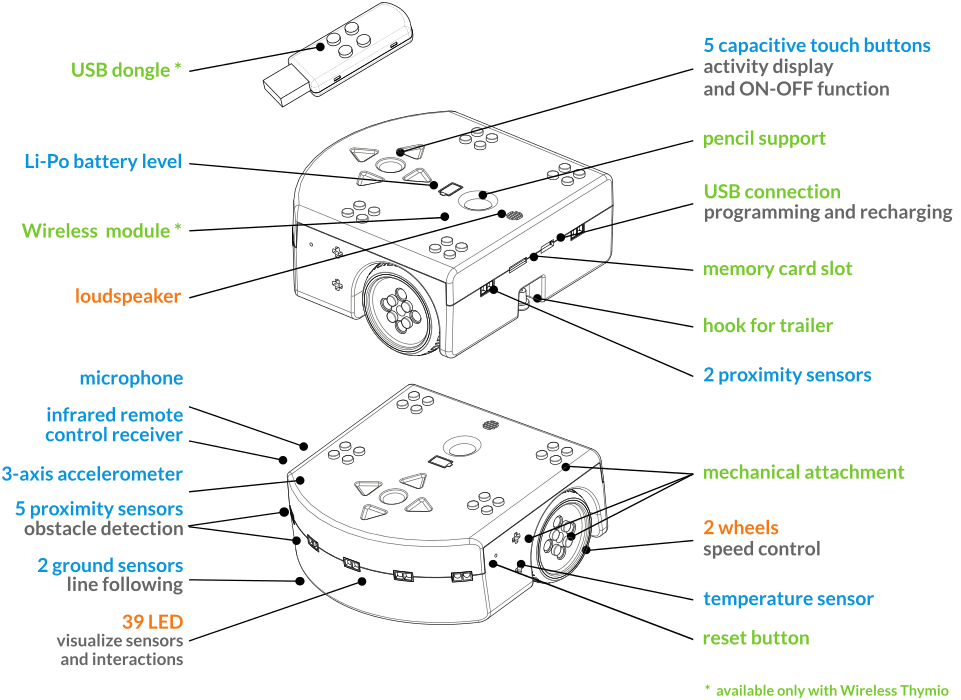
\includegraphics[width=1.0\linewidth]{include/images/thymio.PNG}
  \caption{\label{fig:thymio}Components of Thymio}
\end{minipage}%
\begin{minipage}{.5\textwidth}
  \centering
  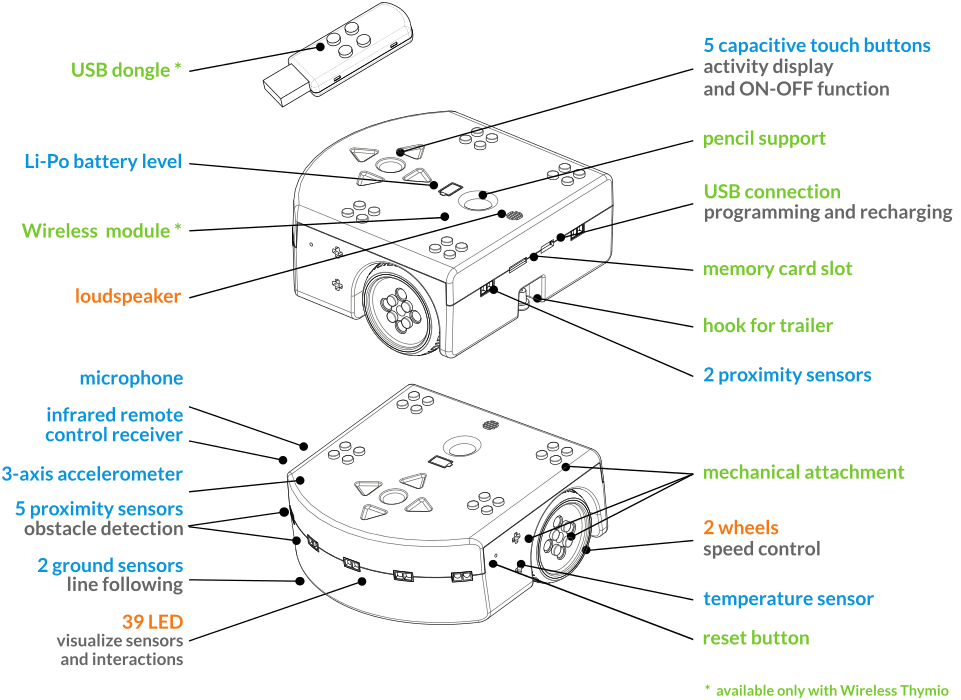
\includegraphics[width=1.0\linewidth]{include/images/thymio.PNG}
  \caption{\label{fig:real_thymio}Thymio II model with attached powerbank}
\end{minipage}
\end{figure}

Thymio robot supports autonomous charging, between 4 and 5 hours of autonomy. In order to evaluate a single evaluation run without any intervetion, we placed a powerbank on top of the thymio. The main characteristics of the Thymio robot is summed up in this table:

\begin{table}[ht]
\centering
\begin{tabular}{|c|L{0.8\textwidth}|}
\hline
Characteristics & \multicolumn{1}{c|}{Values} \\ \hline
\texttt{Length} & 112 mm \\
\texttt{Width} & 117 mm \\
\texttt{Height} & 53 mm \\
\texttt{Weight} & 250 g \\
\texttt{Max. speed} & 0.2 m/s \\
\texttt{IR Sensors} & front.prox.horizontal.[0-4], back.prox.horizontal.[5-6], prox.ground.[0-1]; Proximity sensor response values between range 0-4500;  \\
\texttt{Battery} & Li-Po Battery: 3.7 V, 1'500 mAh, chargeable through microUSB port; Autonomy between 4 and 5 hours \\ \texttt{Powerbank} & 5'500 mAh, chargeable through microUSB port; Autonomy around 23 hours \\ \hline

\end{tabular}
\caption{The main characteristics of the Thymio II model}
\label{tabla_parametros}
\end{table}
\FloatBarrier

\section{Software Architecture}

\subsection{Aseba}

Thymio can be programmed with \emph{Aseba} \cite{retornaz2013seamless}, which is a set of tools that enables to program the robot within several programming environments, namely \emph{Visual, Blockly, Text, Scratch} programming. Aseba is shipped with a command-line utility tool called \emph{asebamedulla}, that allows accessing an Aseba network through \emph{D-BUS}\footnote{\url{https://www.freedesktop.org/wiki/Software/dbus/}}. This enables to program Aseba-enabled devices, the Thymio robot, using third-party languages. Since our preferred language is Python, the python CLI\footnote{\url{https://github.com/aseba-community/aseba/blob/master/examples/clients/python-dbus/aseba.py}} was chosen, which is a thin wrapper around asebamedulla dbus interface.

D-Bus is the main IPC system used in Linux: processes expose objects with a declared interface whose methods can be called from other processes. This is implemented by sending messages over D-Bus itself. The Aseba environment provides a D-Bus interface via the asebamedulla utility, which is in charge of transmitting to the robot hardware. The abstraction is in the form of a network of Thymio robots and processes listening on D-Bus, the so-called \emph{AsebaNetwork}.

The goal of the Aseba D-Bus integration is not to be an alternative to any of the Aseba languages used to program the robots locally. Indeed, it is meant to provide integration with another system, on which not only the D-Bus deamon and asebamedulla are running, but also the programs utilizing the D-Bus interface, which are never transferred in any manner to the Thymio hardware. This, in turn, means that the thymio is continuously connected to the machine on which the Python script, in our case, is running.

The API consists ultimately in the interfaces that asebamedulla provides over D-Bus. Through this interface, we can retrieve information about the network, read and write variables, or send events.

\begin{lstlisting}[style=C-color, caption={The API that asebamedulla provides over D-Bus},label={Asebamedulla API}]

interface ch.epfl.mobots.EventFilter {
    method Void ListenEvent(UInt16 eventId)
    method Void ListenEventName(String eventName)
    method Void IgnoreEvent(UInt16 eventId)
    method Void IgnoreEventName(String eventName)
    signal Event(UInt16 id, String name, Array<SInt16> payloadData)
}

interface ch.epfl.mobots.AsebaNetwork {
    method Void LoadScripts(String fileName)
    method Array<String> GetNodesList()
    method Array<String> GetVariablesList(String nodeName)
    method Void SetVariable(String nodeName, String variableName, Array<SInt16> variableData)
    method Array<SInt16> GetVariable(String nodeName, String variableName)
    method Void SendEvent(UInt16 eventId, Array<SInt16> payloadData)
    method Void SendEventName(String eventName, Array<SInt16> payloadData)
    method ObjectPath CreateEventFilter()
}
\end{lstlisting}

The \emph{AsebaNetwork} interface allows working with all of the nodes (robots) in the same network. There are methods to retrieve a list of the connected nodes ( \emph{GetNodesList} ) and to broadcast a global event, like \emph{SendEvent}. Global events are events that aseba nodes exchange within the aseba network. On the other hand, events that are internal to the node are called \emph{local events}. \emph{SetVariable} and \emph{GetVariable}, which write and read respectively native variables of the Aseba scripting language.

Asebamedulla exposes the interface \emph{EventFilter} which allows managing events. An application that wants to listen to events have register events with \emph{ListenEventName} or \emph{ListenEvent} be notified when an event occurs. The application can receive these events through the \emph{Event} signal, these events correspond to the global events of the Aseba language.

\subsection{Robotic Simulator}

In our experiments, a set of tools is needed in order to develop, test and validate different approaches to the reality gap problem. In relation to evolutionary robotics, these tools represent robotic simulators and robotic frameworks. Robotic simulators help to build the bridge between simulation and reality, they endorse that the developed simulation can be transferred and applied to real robotics. The most well know simulators in the community are \emph{V-REP} \cite{rohmer2013v} and \emph{Gazebo} \cite{koenig2004design} based on a survey made by Ivaldi, Peters, \cite{ivaldi2014tools}. These two simulators are compared in basic robotic control logic and evolutionary robotics experiment in \cite{nogueira2014comparative}. \emph{V-REP} robot simulation framework came out as the more intuitive and user-friendly simulator, which comes with various features and is less hardware demanding. Moreover, we have experience with \emph{V-REP} from previous works, therefore it was chosen as our main robotic framework.

In this work the use of V-REP simulation is not only used for \emph{Simulation-based optimization} and \emph{Robot-in-the-loop simulation-based optimization} approaches but also for \emph{Reality-based optimization} approach. V-REP exposes a remote API that allows controlling the simulation from the external client-side application. The client-side application is written in python which enables to control the simulation over the simulation variables.

\subsection{Computer Vision}

One of the most pivotal points of the computer vision is to track the Thymio robot during evaluation and positioning of the obstacles in the simulation. Therefore it goes without saying that the system must be able to accurately read the position and angle of these objects. Since the environment is static and small in size, a fixed-camera computer vision is optimal to extract the necessary spatial information within a single image. The most necessary problem is solving the objects identification and accurate spatial information extraction. These problems are usually dealt with using certain marker systems. One of such a system is \cite{bencina2005improved}, which relies on 2D tracking of specially designed fiducials (markers) in a real-time video stream. This system involves a set of marker patterns and computer vision algorithms that can track and yield various spatial information of these markers. Such a marker system was chosen for our needs. The choice is supported by the same computer vision system being used and proven in \cite{faina2017automating}.

\subsubsection{Fiducial tracking}

The \epmh{ReacTIVision Fiducials}\ref{fig:fiducial_markers} comes in 3 different set of sizes \emph{small, medium, large} and each individual marker has it's own unique id. Furthermore, each of them is purely identified by its unique topological structure. The system employs the topological fiducial recognition, which enables detection and identification. In this approach, a region adjacency graph is computed from a binary image. The adjacency graph can be understood as a tree. By recognizing the graphs representing the fiducials, markers can be detected and identified. Moreover, the location is computed as the weighted average of all leaf centers (black and white). The vector from this centroid to a point given by the weighted average of all black (or white) leaf centers is used to compute the orientation of the fiducial \cite{bencina2005improved}.

\begin{figure}[H]
  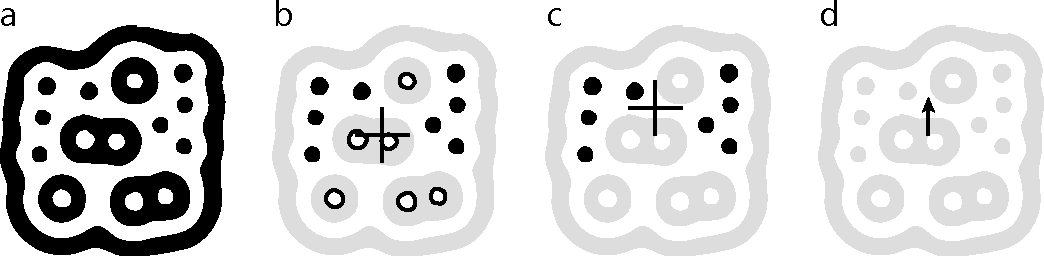
\includegraphics[width=0.66\linewidth]{include/images/fiducial_markers.PNG}
  \caption{\label{fig:fiducial_markers}ReacTIVision Fiducials from original paper a) a reacTIVision fiducial (b) black and white leafs and their average centroid (c) black leafs and their average centroid, and (d) the vector used to compute the orientation of the fiducial}
\end{figure}

\subsubsection{Computer Vision Implementation}

\subsection{Path Following}

\section{Automation Control}

\subsection{Evaluation of the robotic platform}
